\chapter{Análise de resultados}

Nesse capítulo, serão apresentados os dados, obtidos através da simulação, e realizada uma análise para avaliar as diferentes configurações utilizadas e seus impactos na fluxo do tráfego em um cruzamento. Os parâmetros adquiridos das simulações foram a duração da viagem de cada veículo em cada caminho (do ponto de partida até o ponto de chegada) e o tempo de espera em fila de cada caminho. Esses dados são adquiridos a cada passo da simulação, e utiliza os dados de todos os veículos que passam por cada caminho, sendo assim os dados calculados desde o início da simulação, até que nenhum carro seja mais emitido.

Como já foi apresentado no capítulo referente à simulação, os seguintes cenários foram analisados:

\begin{itemize}
\item 1 - Cruzamento sem a utilização do sistema.
\item 2 - Cruzamento com o sistema, utilizando uma programação de tempos fixos.
\item 3 - Cruzamento com o sistema, agindo de modo adaptativo, com o auxílio de um detector em uma via.
\item 4 - Cruzamento com o sistema, agindo de modo adaptativo, com o auxílio de dois detectores, em vias distintas, identificando o fluxo nas direções ortogonais. %vertical e horizontal
\end{itemize}

Para filtrar os dados desejados dos arquivos exportados, foi escrito um script, em python, que realiza uma varredura, em arquivos do tipo xml, e obtem os dados necessários. Esse script também processa esses dados, gerando os valores e gráficos analisados nesse capítulo.

\section{Duração da viagem}

Para cada simulação, foram obtidos os dados da duração da viagem de cada veículo emitido em cada percurso estabelecido no cenário. Com esses dados foi possível traçar um gráfico para cada caminho, representando o tempo de viagem para se completar tal percurso, a cada passo da simulação. Desse modo, foi possível traçar quatro gráficos, para cada simulação, representando esses valores, além de contruir uma tabela exibindo as médias de cada percurso, possibilitando uma comparação direta entre os cenários.

A Tabela \ref{tab: duration} apresenta os valores médios da duração de cada viagem, por caminho, demonstrando qual utilização do sistema apresentou maior impacto positivo sobre o cenário. Esses dados serão relacionados com os gráficos traçados, para uma análise mais completa desse parâmetro.

\begin{table}[H]
\centering
\caption{Duração da viagem (s)}
\label{tab: duration}
\begin{tabular}{@{}llllll@{}}
\toprule
Cenário & Caminho 1 & Caminho 2 & Caminho 3 & Caminho 4 & Total \\ \midrule
1 & 179 & 180 & 180 & 178 & 179 \\
2 & 58 & 62 & 57 & 63 & 60 \\
3 &	63 & 57 & 61 & 57 & 59 \\
4 & 67 & 57 & 63 & 56 & 61 \\
\bottomrule
\end{tabular}
\end{table}

Como o objetivo do sistema é organizar o trânsito, de maneira a melhorar a experiência de todos os usuários (motoristas, passageiros, pedestres), a duração da viagem é um dado que se relaciona diretamente com tal organização, com uma relação inversamente proporcional.

Os gráficos das Figuras \ref{tripNoTL} a \ref{tripTwoLoop} apresentam os dados referentes à duração da viagem, de cada simulação. 

\begin{figure}[H]
    \begin{center}
    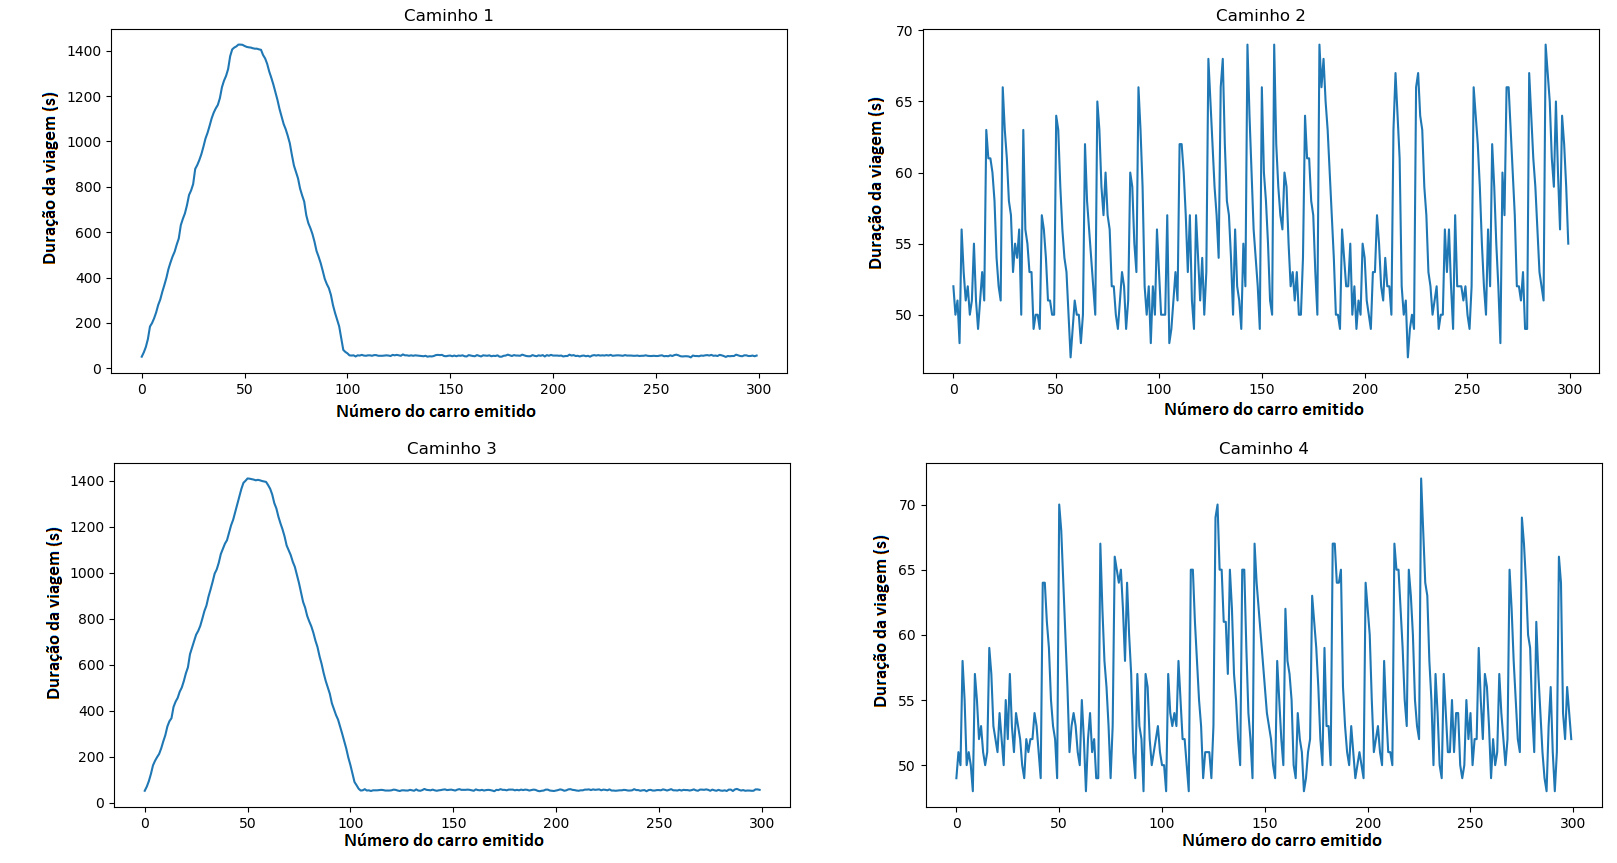
\includegraphics[width=1\textwidth]{figuras/Trip_Duration_No_TrafficLight.PNG}
    \end{center}
    \caption[Duração da viagem, cenário 1]{Simulação sem o sistema.}
    \label{tripNoTL}
\end{figure}

\begin{figure}[H]
    \begin{center}
    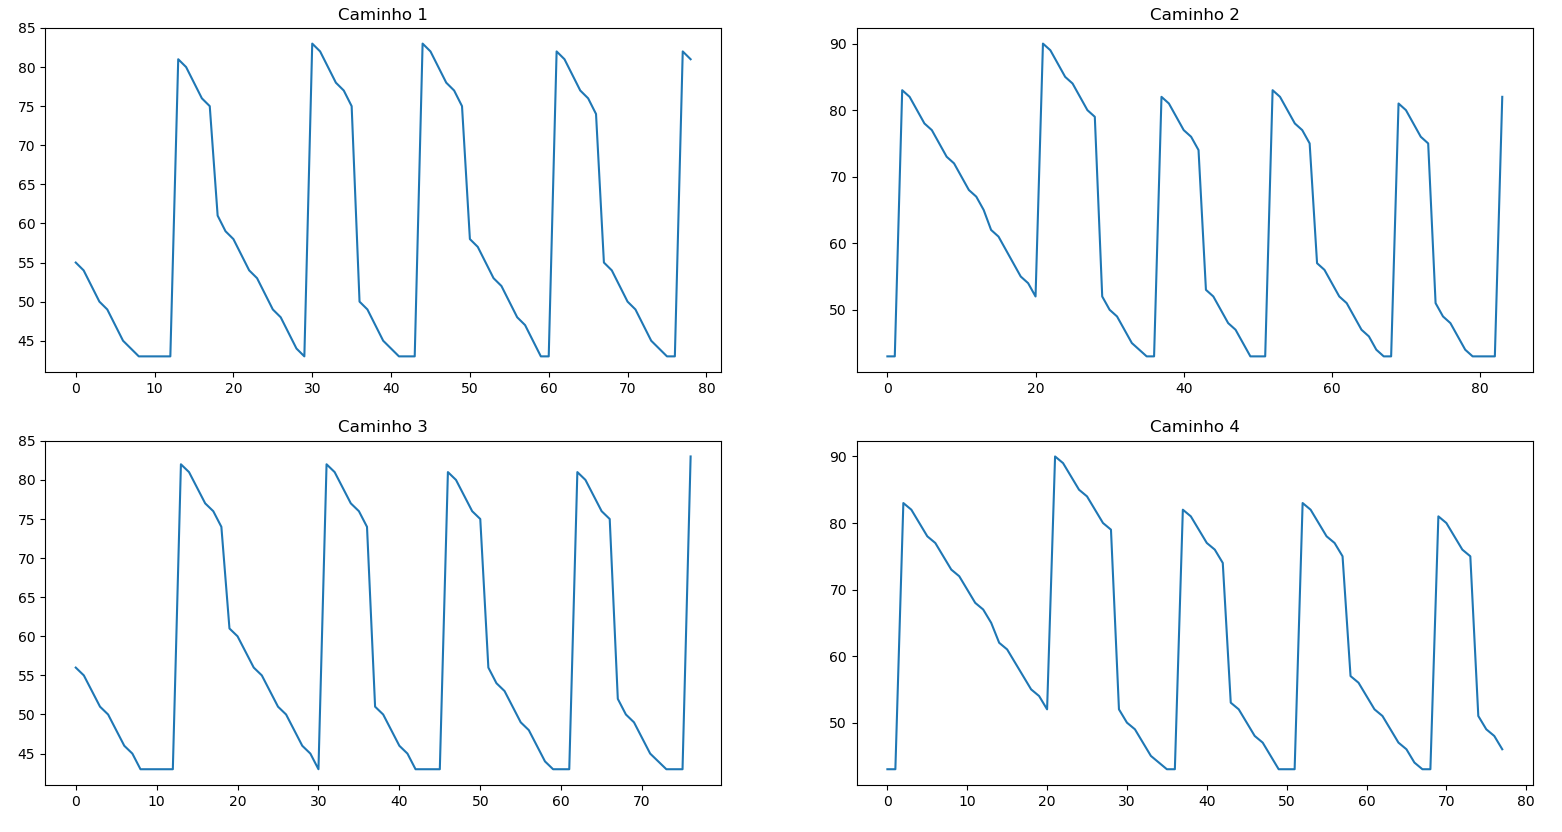
\includegraphics[width=1\textwidth]{figuras/Trip_Duration_With_TrafficLight.PNG}
    \end{center}
    \caption[Duração da viagem, cenário 2]{Simulação com o sistema funcionando com tempos fixos.}
    \label{tripWithTL}
\end{figure}

\begin{figure}[H]
    \begin{center}
    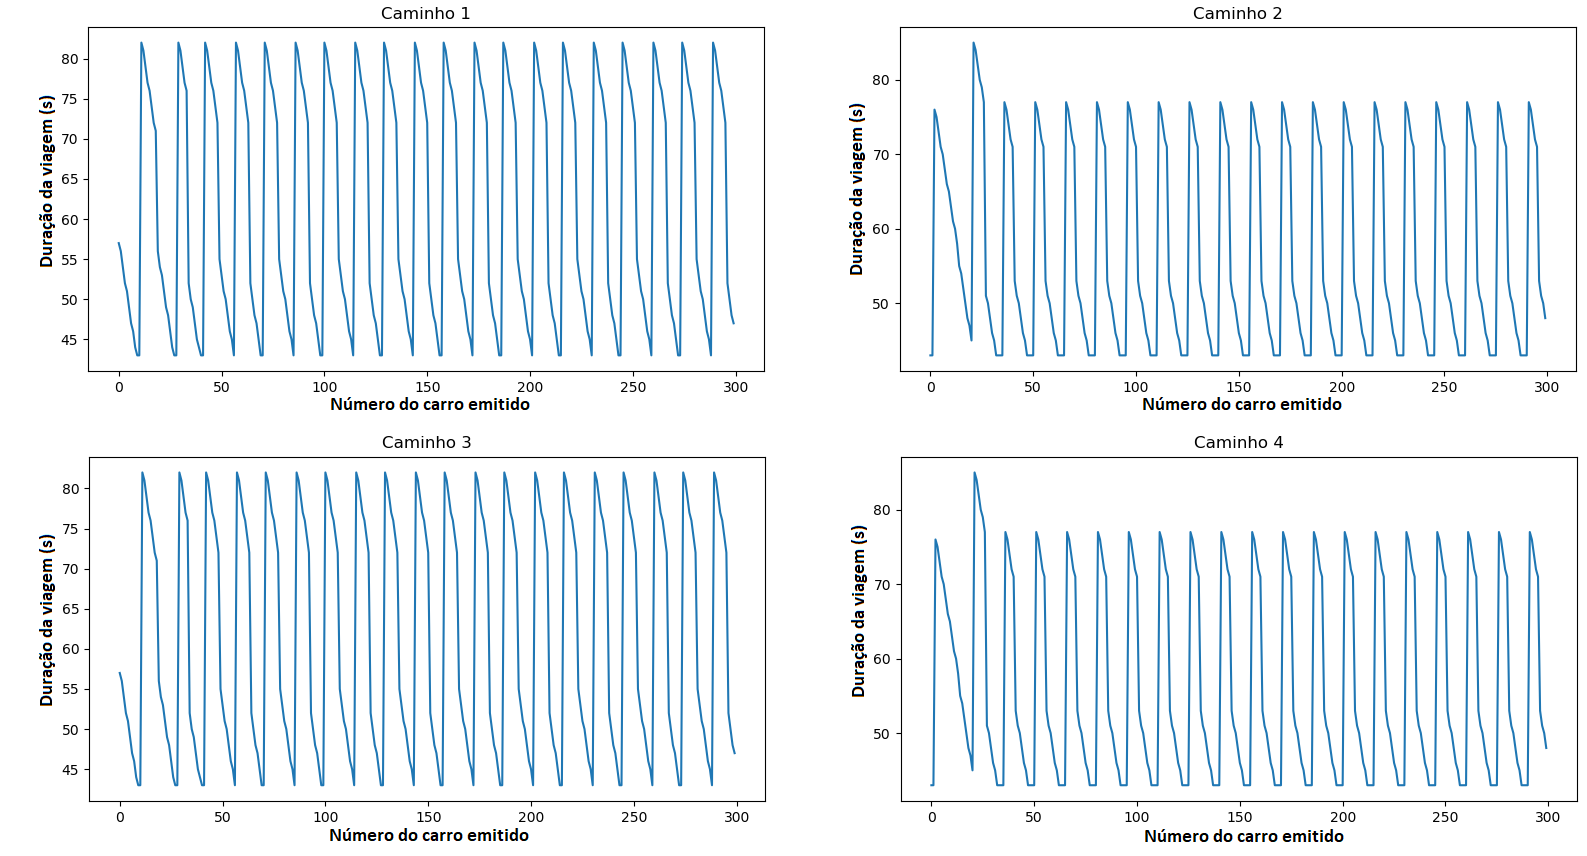
\includegraphics[width=1\textwidth]{figuras/Trip_Duration_With_One_Loop.PNG}
    \end{center}
    \caption[Duração da viagem, cenário 3]{Simulação com o sistema adaptativo com um laço.}
    \label{tripOneLoop}
\end{figure}

\begin{figure}[H]
    \begin{center}
    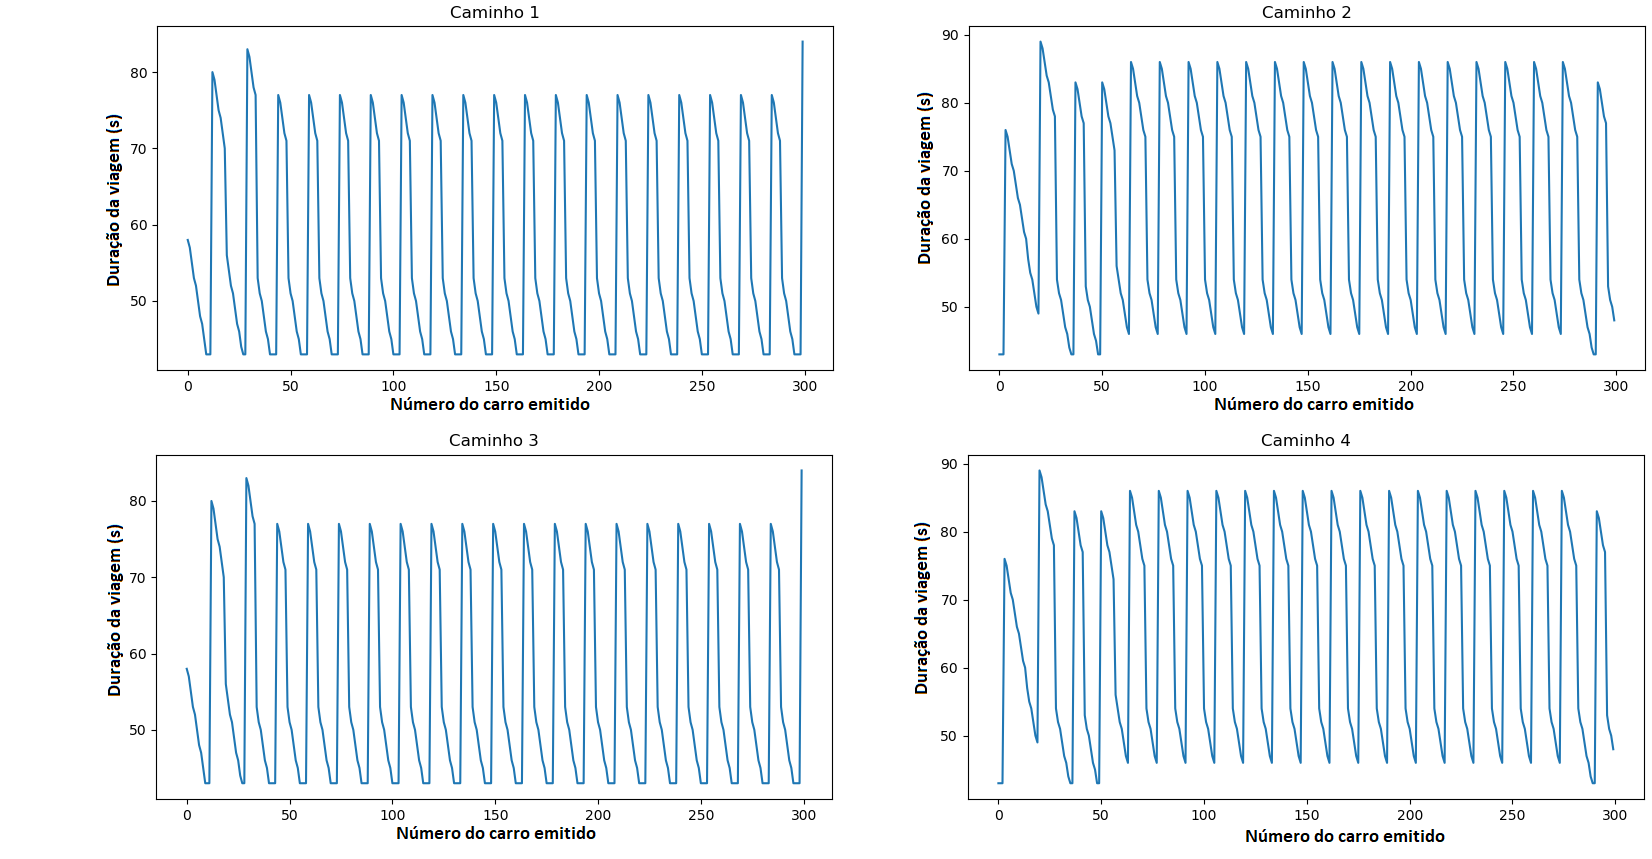
\includegraphics[width=1\textwidth]{figuras/Trip_Duration_With_Two_Loop.PNG}
    \end{center}
    \caption[Duração da viagem, cenário 4]{Simulação com o sistema adaptativo com dois laços.}
    \label{tripTwoLoop}
\end{figure}

\section{Tempo de espera em filas}
Seguindo a mesma metodologia de obtenção dos dados referentes à duração das viagens, foram coletados dados referentes ao tempo esperado em filas, para cada caminho. Esse dado é calculado, a cada passo da simulação, medindo a distância entre o ponto de referência (em todos os casos, esse ponto foi o node 0 da simulação, ou o cruzamento em si) e o último carro parado no caminho determinado.

Novamente, com os dados obtidos a partir da simulação, foi possível construir a Tabela \ref{tab: queue} com os valores das médias do parâmetro, assim como traçar um gráfico para cada caminho, em cada cenário.

\begin{table}[H]
\centering
\caption{Tempo de espera em filas (s)}
\label{tab: queue}
\begin{tabular}{@{}llllll@{}}
\toprule
Cenário & Caminho 1 & Caminho 2 & Caminho 3 & Caminho 4 & Total \\ \midrule
1 & 102 & 104 & 105 & 105 & 104 \\
2 & 18 & 23 & 17 & 17 & 21 \\
3 &	25 & 20 & 24 & 20 & 22 \\
4 & 29 & 18 & 23 & 17 & 22 \\
\bottomrule
\end{tabular}
\end{table}

Os gráficos das Figuras \ref{queueNoTL} a \ref{queueTwoLoop}  apresentam os dados referentes ao tempo de espera em filas, das quatro simulações.

\begin{figure}[H]
    \begin{center}
    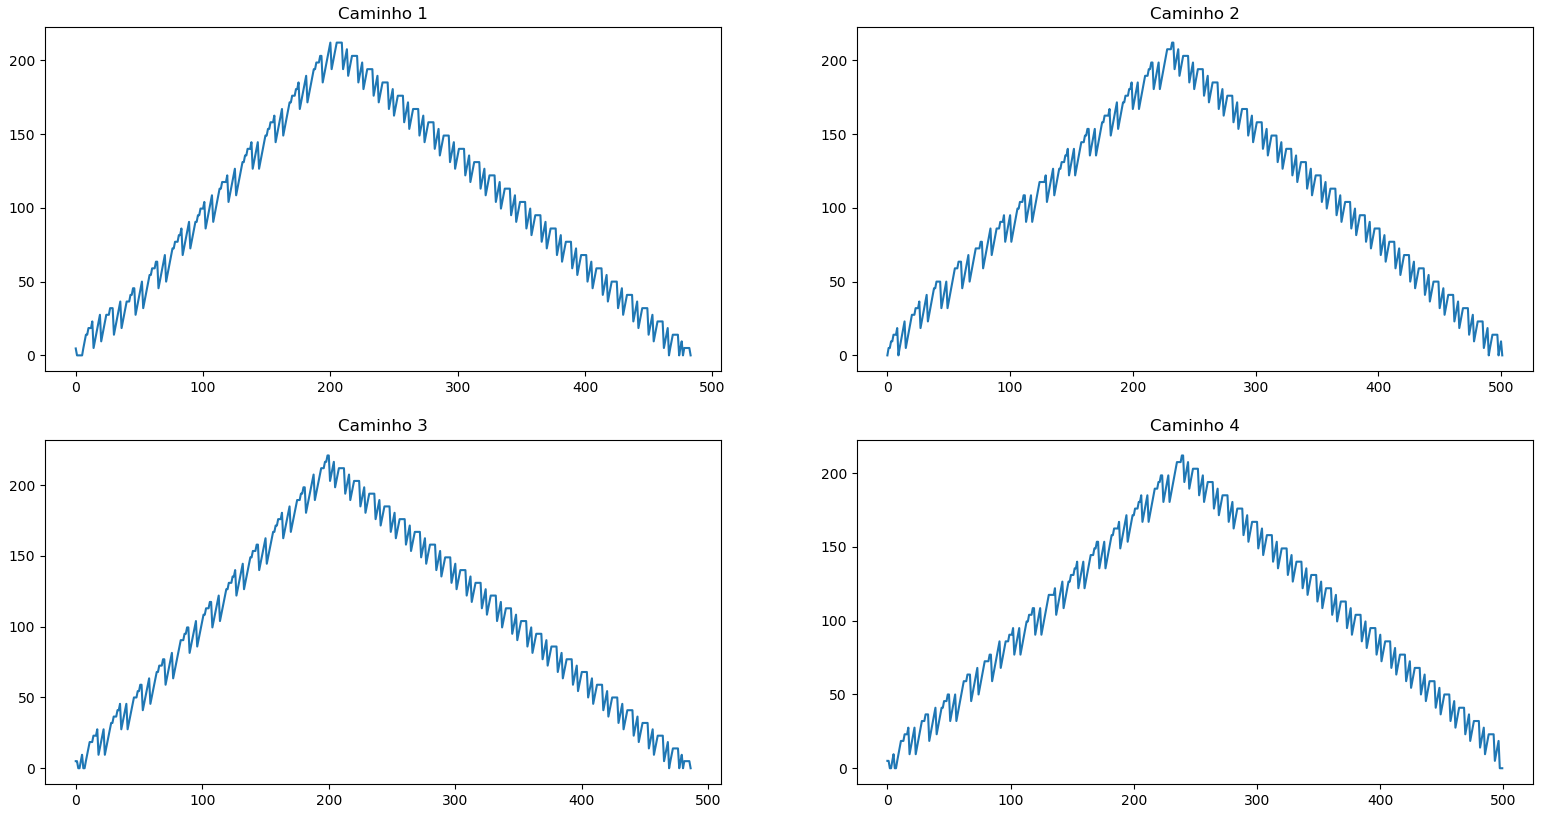
\includegraphics[width=0.8\textwidth]{figuras/Queue_Duration_No_TrafficLight.PNG}
    \end{center}
    \caption[Duração das filas, cenário 1]{Simulação sem o sistema.}
    \label{queueNoTL}
\end{figure}

\begin{figure}[H]
    \begin{center}
    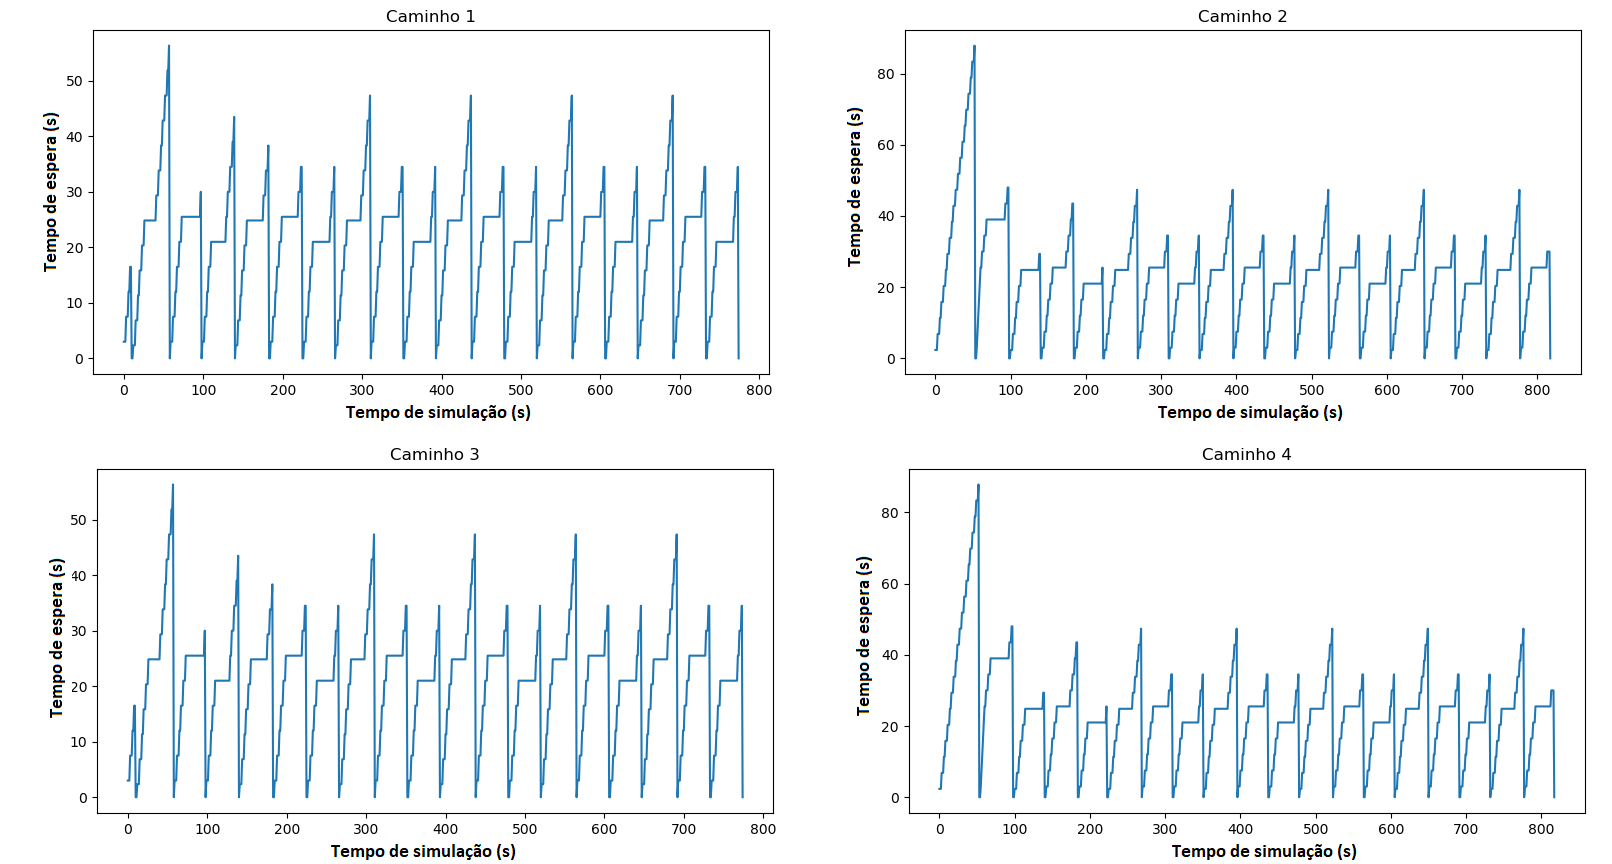
\includegraphics[width=0.8\textwidth]{figuras/Queue_Duration_With_TrafficLight.PNG}
    \end{center}
    \caption[Duração das filas, cenário 2]{Simulação com o sistema funcionando com tempos fixos.}
    \label{queueWithTL}
\end{figure}

\begin{figure}[H]
    \begin{center}
    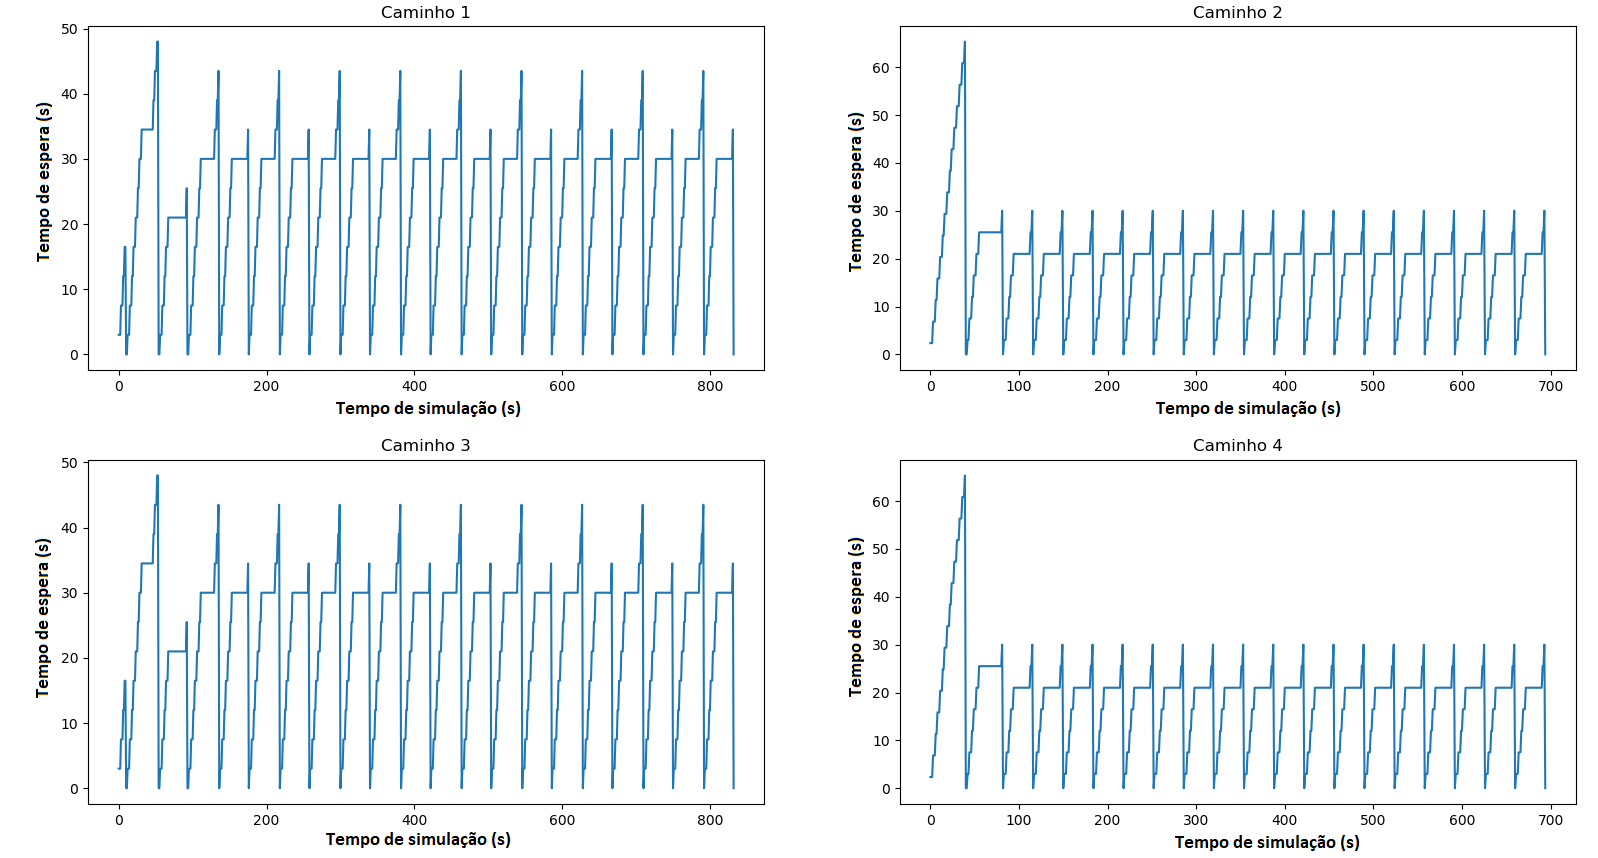
\includegraphics[width=0.8\textwidth]{figuras/Queue_Duration_With_One_Loop.PNG}
    \end{center}
    \caption[Duração das filas, cenário 3]{Simulação com o sistema adaptativo com um laço.}
    \label{queueOneLoop}
\end{figure}

\begin{figure}[H]
    \begin{center}
    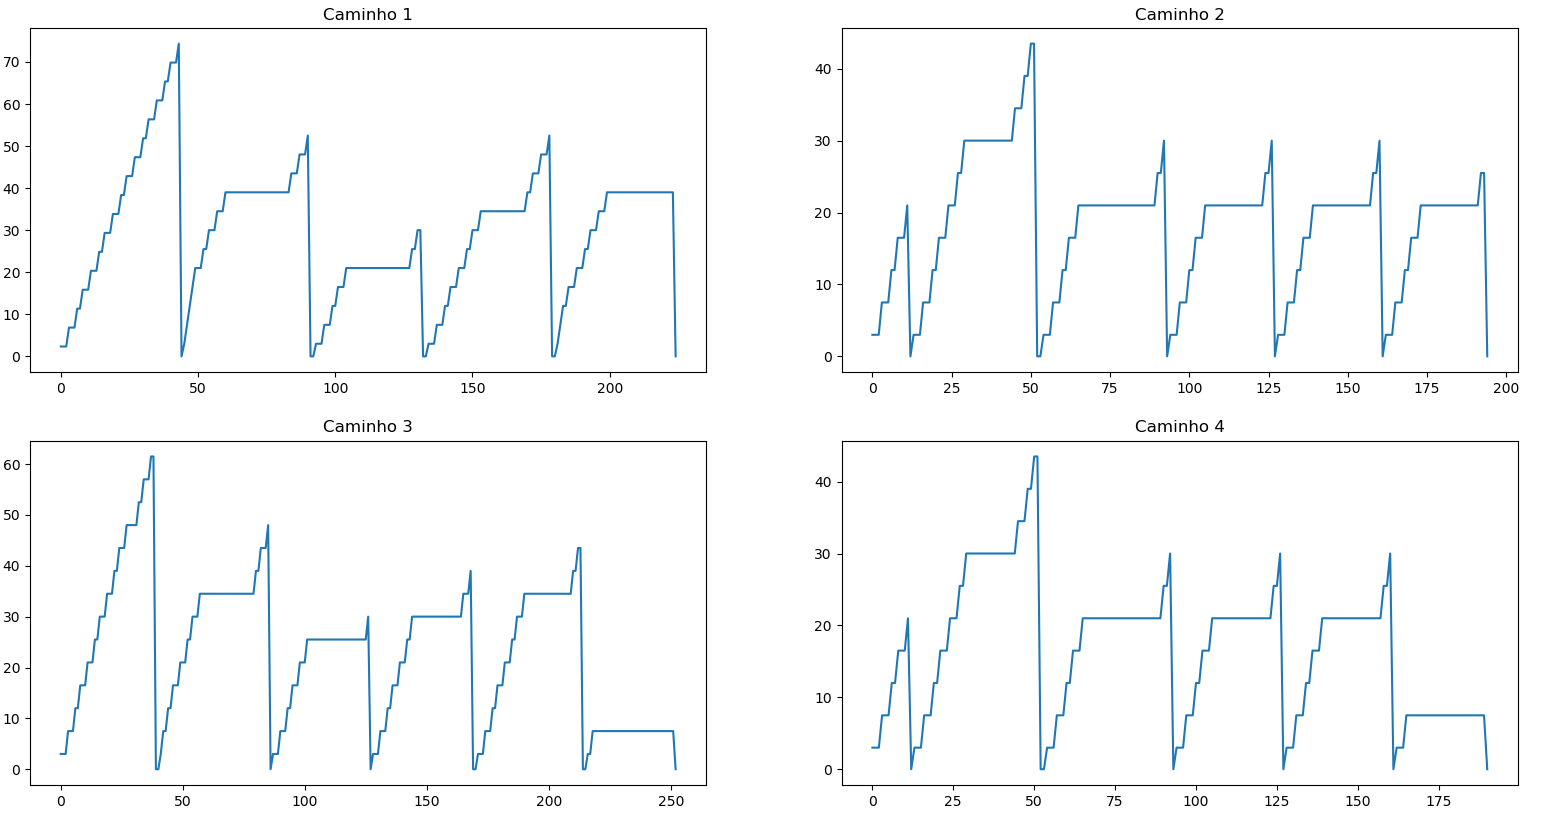
\includegraphics[width=0.8\textwidth]{figuras/Queue_Duration_With_Two_Loop.PNG}
    \end{center}
    \caption[Duração das filas, cenário 4]{Simulação com o sistema adaptativo com dois laços.}
    \label{queueTwoLoop}
\end{figure}

\section{Desempenho do sistema}

Ao observar os valores das tabelas, percebe-se que a implementação do sistema teve um impacto bastante positivo no fluxo de veículos. No caso da duração da viagem, houve uma redução de até $68,54\%$, se comparados os valores do caminho 4 para os cenários 1 e 4. Já no caso do tempo de espera em filas apresentou uma redução de até $83,81\%$, comparando os valores do caminho 4, para os cenários 1 e 2 (essa mesma melhoria foi observada em outros cenários). Ainda se forem observados os piores casos, há uma redução de $62,57\%$ no tempo de viagens, e $71,57\%$ no tempo de espera nas filas.

Observando os gráficos, é fácil reconhecer, tanto na duração da viagem, quanto no tempo de filas, que há um padrão no comportamento do fluxo veicular, quando o sistema está em funcionamento. Percebe-se isso comparando os gráficos dos cenários 2, 3 e 4. 

No caso da duração das viagens, os gráficos mostram tempo de viagem (s) por veículo emitido naquele caminho. 
Nota-se, nos gráficos do primeiro cenário, que esse parâmetro não diminui durante toda a simulação, ultrapassando o valor de 300 s, próximo ao final. Cada carro emitido no caminho apresenta um tempo de viagem maior que os anteriores, isso representa a formação de trânsito. 
Nos cenários 2, 3 e 4, porém, nota-se que os gráficos seguem um comportamento semelhante, em que o tempo de viagem sofre um leve aumento, durante o período de semáforo fechado, mas volta a cair quando ocorre a abertura. Nenhum caminho, de nenhum cenário, apresentou duração de viagem superior a 100 s, demonstrando a eficácia do sistema. 

No caso do tempo de espera em filas, os gráficos mostram tempo em filas (s) por tempo de simulação (s). O primeiro ponto a ser notado é que, no primeiro cenário, os gráficos apresentam muito mais valores de tempo de simulação. Isso é devido à formação de trânsito, fazendo com que os veículos precisem de mais tempo para completar o percurso. Ainda no gráfico do primeiro cenário, é possível visualizar o momento em que os carros param de ser emitidos na simulação, observado pelo início do declínio do tempo das filas.
Nos cenários 2, 3 e 4, observa-se um comportamento semelhante aos gráficos de duração da viagem, onde o parâmetro sofre um aumento durante o tempo de semáforo fechado, seguido por uma melhora, quando o fluxo é liberado.

Com esses resultados, é possível notar que existe uma correlação entre os dois parâmetros observados. Âmbos apresentaram uma melhoria significativa com a implementação do sistema. A duração do percurso é limitada pelo tempo de abertura do semáforo, enquanto o tempo em filas (efetivamente o tempo que o veículo passa parado) é limitado pelo tempo em que o semáforo permanece fechado.

Uma observação a ser feita, é que não houve melhoria no sistema, ao aumentar a quantidade de detectores utilizados. Isso se deve pela simplicidade do cenário, pois o detector é utilizado para trocar a prioridade da via, e com apenas duas fases do semáforo, apenas um detector é suficiente para realizar o controle semafórico. 